\documentclass{article}
\usepackage{geometry}
\geometry{a4paper}
\usepackage{listings}
\usepackage{graphicx} 
\usepackage[ngerman]{babel}
\usepackage[utf8]{inputenc}
\usepackage[T1]{fontenc}    
\usepackage{amsmath}
\usepackage{float}
\usepackage{url}

\title{
	Bericht: Simulation von Bewegungen \\
	\large Raumsonde mit steuerbarem Antrieb: Flug zu einem Planeten}
\author{Amin Nacer Cherif, Simon Wohler, Joel André}

\begin{document}

\maketitle

\section{Auftrag}
In unserem Projekt geht es darum, dass man im Sonnensystem, von der Erde aus, eine Raumsonde gezielt auf, bzw. in die Umlaufbahn eines anderen Planeten(z.B. Saturn) schiessen kann. Dabei soll ein swing-by Manöver um einen dazwischenliegenden Planeten(z.B. Jupiter) vollführt werden.

	\subsection{Persönliche Ziele}
		\begin{itemize} 
			\item Simulation des Sonnensystems
			\item Zwei verschiedene Modi
			\begin{itemize} 
				\item Manuell steuerbare Raumsonde
				\item Raumsonde fliegt festgelegtes swing-by Manöver
			\end{itemize}
		\end{itemize}

\section{Motivation}
Gewählt wurde das Thema, weil es eine Herausforderung darstellt und gleich mehrere zu lösende Probleme auf einmal enthält. Zudem sind wir eine Gruppe aus drei Personen, wodurch es möglich ist, eine Problemstellung mit grösserem Umfang zu bearbeiten. Alle Gruppenmitglieder empfinden das Thema als spannend und interessant.

\section{Vorgehen und Reflexion}
Als erster Schritt wurde festgehalten, welche Teilschritte gemacht und Module erstellt werden müssen. So wusste immer jeder, was es noch zu erledigen gibt und konnte sich nach einem abgeschlossenen Schritt direkt dem Nächsten widmen. 
Dazu wurden \textit{Github Issue's} verwendet. 

Amin hatte dann begonnen das \textit{Runge-Kutta} Verfahren zu programmieren. Dabei hatten wir anfängliche Verständnis-Schwierigkeiten, bezüglich dem Aufstellen der DGL.
Gleichzeitig widmete sich Joel, unter anfänglicher Unterstützung Simons, dem Programmieren eines Sonnensystems mit \textit{Pygame}. Dazu hat Simon nach Anfangsbedingungen für das Sonnensystem gesucht. Als Schwierigkeit stellte sich dabei die Berechnung der Anfangsgeschwindigkeiten der Planeten heraus. Durch Herr Kambors physikalische Unterstützung konnten diese jedoch sehr genau berechnet werden. 

Als nächstes begann Amin damit ein Menu zu programmieren, während Joel das fertiggestellte \textit{Runge-Kutta} Verfahren in das main-Programm implementierte. Schnell schien die Simulation zu funktionieren, da sich die Planeten für eine kurze Zeit korrekt bewegten. Allerdings nahm ihr Abstand zur Sonne stetig zu, was eindeutig nicht sein sollte. Der Fehler wurde nicht gleich gefunden, doch konnte festgestellt werden, dass er irgendwo im Programmcode steckt, denn die Anfangsbedingungen wurden alle nochmals überprüft und mit den Angaben der NASA verglichen. Herausgestellt hat sich dann, dass es lediglich ein Flüchtigkeitsfehler war und in der Differenzialgleichung auf alte Positionen zugegriffen wurde.
Danach wurde das Menu implementiert, in welchem man auswählen kann, ob man die Rakete selbst steuert oder ob ihr Flug simuliert werden soll. Als weitere Funktion kann man im Menu einige wichtige Parameter festsetzen. Dies funktionierte aber noch nicht, denn trotz eingegebenen Daten ändert sich überhaupt nichts an der Simulation. Joel widmete sich dann dem Schreiben einer Zoom-Funktion, mit welcher man direkt auf einen Planeten zoomen kann. Parallell dazu hat Simon eine Funktion geschrieben, damit man manuell bestimmen kann wie schnell die Zeit in der Simulation vergeht. 
Als letzter Schritt wurde der ganz Programmcode nochmals sorgfältig überarbeitet und kommentiert.

\section{Produkt (aktueller Stand)}
\begin{figure}[hbt]
	\centering
		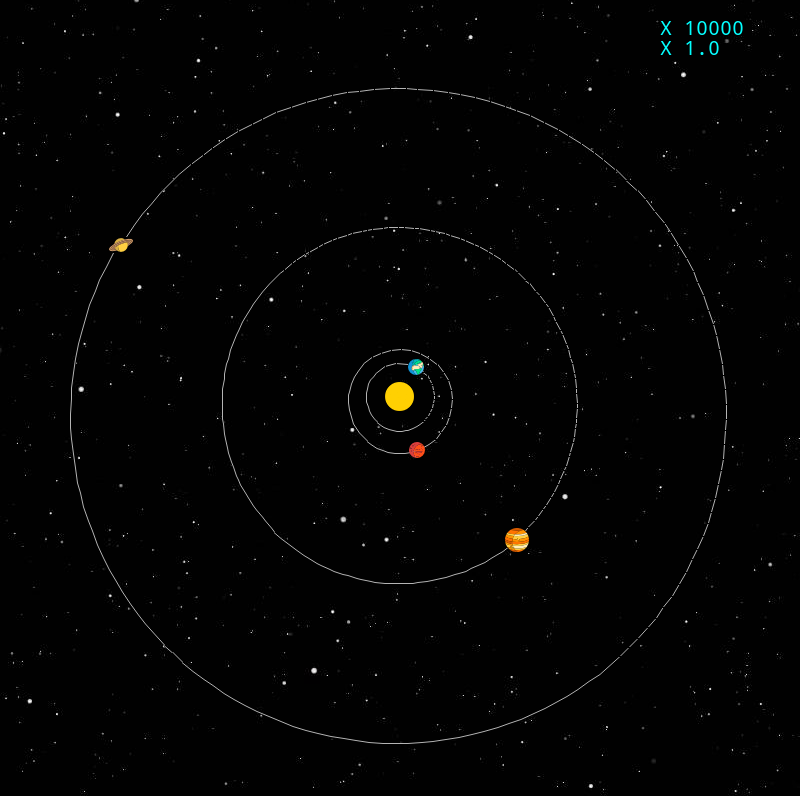
\includegraphics[width=0.8\textwidth]{game.png}
	\caption{Simulation}
	\label{img:simulation}
\end{figure}
\subsection{Simulation des Sonnensystems}
Aktuell kann das Programm erfolgreich das Sonnensystem mit ausgewählten Planeten simulieren. Simuliert werden Erde, Mars, Jupiter und Saturn. Die Anfangsbedingungen stimmen sehr genau mit dem Sonnensystem überein.
\subsubsection{Implementation des \textit{Runge-Kutta }Verfahrens}
Das \textit{Runge-Kutta} Verfahren wird lediglich einmal, jedoch gleich für alle Planeten durchgeführt. Das liegt daran, dass bei einem Schritt auch die neuen Positionn der anderen Planeten berücksichtigt werden muss.

In der DGL werden zuerst alle Beschleunigungen addiert, die auf einen Körper wirken.
\subsection{Interface}
\subsubsection{Menu}
Ein Menu wurde ebenfalls implementiert. Allerdings ist es noch voller kleiner, versteckter Fehler. Es gibt momentan schon viele Knöpfe, aber viele sind noch ohne Funktion. Später soll man dann zwischen den Modi wechseln können und Konstanten ändern.
\subsubsection{Zoom}
Ein Zoom war wichtig für die Raumsonde. Ohne Zoom wäre es unmöglich, die Sonde in Erdnähe präzis zu steuern. Wenn man mit der Maustaste auf Körper drückt, kann man das Zentrum der Simulation ändern. So ist es dann möglich, auf einen einzelnen Planeten zu zoomen.

\textit{p} vergrössert und \textit{m} verkleinert
\subsubsection{Geschwindigkeit}
Der Geschwindigkeitsfaktor wird realistisch angezeigt. Das Spulen nach vorne war ebenfalls nötig, um bei langsamer Geschwindigkeit die Sonde zu steuern, und dann bei schneller Geschwindigkeit Resultate zu sehen.

\textit{arrow up} beschleunigt und \textit{arrow down} verlangsamt.

\subsubsection{Spur}
Eine Spur wurde zur Übersichtlichkeit hinzugefügt. Die Länge der Spur lässt sich als Zeit [s] einstellen. Momentan hat die Spur bei allen Planeten die Länge des Umfangs ihrer Umlaufbahn. Dass die Spur sich schön schliesst, beweist, dass die Umlaufzeit der Planeten mit der echten Umlaufzeit übereinstimmt.


\section{Reflexion und Ausblick}
Rückblickend sind wir uns einig, dass die Organisation in der Gruppe ziemlich gut funktioniert hat. Jeder hatte immer etwas zu tun und durch erfolgreiche Kommunikation habe wir immer gemeinsam auf ein Zwischenziel hin gearbeitet. Am schwierigsten war es, einmal eine funktionierende Simulation zu programmieren inklusive dem implementierten \textit{Runge-Kutta} Verfahren. Alle Ergänzungen danach fielen uns einiges leichter. 


Der nächste Schritt in unserer Arbeit wird sein, die Raumsonde zu simulieren. Dazu wird sie der gleichen Klasse zugewiesen, wie die anderen Planeten auch. 
D.h. sie wird wie ein mini Planet behandelt. Die Raumsonde ist mit einem \textit{Vulcain 2} Triebwerk ausgestattet und sollte in der Simulation auch dementsprechend viel Schub haben. 
$$ a = \frac{F_{Vulcain2}}{M_{Vulcain2} + M_{Sonde}} $$
Zudem sollte die Raumsonde gesteuert werden können, indem man den Winkel, in welchem die Rakete fliegt, ändern kann. Vorgesehen ist, dass als Anfangswert die Raumsonde direkt an der Erde fixiert wird. 

Um beim Steuern abschätzen zu können, in welche Richtung die Raumsonde fliegt, werden wir versuchen eine Spur vor der Raumsonde anzeigen zu lassen. Diese Spur wird zeigen, wo die Raumsonde hinfliegen würde, falls nicht beschleunigt wird.

Das Wunschziel unserer Gruppe ist es, zuletzt noch ein kleines Programm zu schreiben, welches direkt die optimale Route zu einem anderen Planeten berechnet und dies optimalerweise auch mit Hilfe eines swing-by Manövers.

\end{document}
